Table \ref{tab:budget} shows the budget for this study.
The meteorological data for the initial and boundary conditions as well as the simulation model are both free.
They are available to download on the internet.
The PC Workstation is available in the laboratory.
Printing and bookbinding is estimated to be 500 Philippine Pesos,
and will be the only cost for the study.

\begin{table}
	\caption{Budget for this study.}
	\label{tab:budget}
	\centering
	\begin{tabular}{l r}
		\hline \hline
		Item & Price (PHP) \\
		\hline
		Meteorological data	& 0 \\
		RegCM & 0 \\
		PC Workstation & 0 \\
		Printing and bookbinding & 500 \\
		\hline
		\textbf{Total} & \textbf{500} \\
		\hline
	\end{tabular}
\end{table}

Figure \ref{fig:timeline} shows the timeline for this study.
Term 1 of Academic Year 2024-2025 will be dedicated to the proposal of the study and the preparation to run the simulations.
The proposal of this study is expected to be conducted by October.
After the proposal, meteorological data for the initial and boundary conditions for the data will be downloaded.
With the large file size, it is expected to take a while to download it.
Term 2 of Academic Year 2024-2025 will be dedicated to the running of simulations and the analysis of the results.
Term 3 of Academic Year 2024-2025 will be dedicated to finishing the manuscript and defending the study.

\begin{figure}
	\centering
	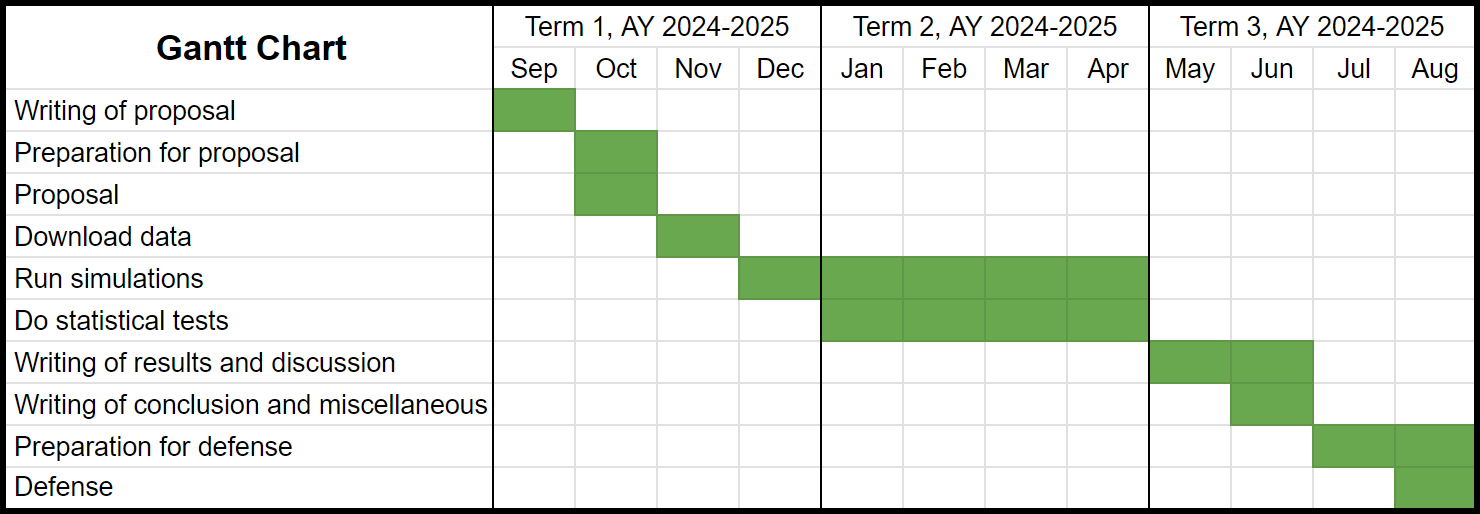
\includegraphics[width=\textwidth]{proposal-gantt-chart}
	\caption{Timeline for this study.}
	\label{fig:timeline}
\end{figure}